\chapter{Oxydation et réduction en chimie organique}\label{ch:b1:organic-redox}

Une bouteille de vin restée ouverte se change en quelques jours en
vinaigre~: des bactéries utilisent le dioxygène de l'air pour oxyder
l'éthanol en acide éthanoïque. Une cétone et l'alcool dont elle provient
diffèrent de deux atomes d'hydrogène --- et, si l'on compte bien, de
deux électrons. Les oxydations et réductions organiques ne ressemblent
pas aux échanges d'électrons entre ions métalliques du
\cref{ch:b1:nernst}, car les électrons voyagent avec des protons ou avec
des ions hydrure, mais la comptabilité est la même. Ce chapitre attribue
des \omterm{def:b1:organic-redox:oxidation-level}{niveaux d'oxydation} au carbone, s'en sert pour prévoir ce que donne
chaque alcool par oxydation, et présente les hydrures qui réduisent les
composés carbonylés, en regardant quels groupes chaque réactif laisse
intacts.

\begin{recall}
Les \omterm{def:b1:nernst:oxidation-number}{nombres d'oxydation}, les \omterm{def:b1:nernst:couple}{demi-équations} et l'écriture des équations
d'oxydoréduction sont au \cref{ch:b1:nernst}~; les classes d'alcools et
de carbones au \cref{ch:b1:electronic-effects}~; les \omterm{def:b1:acetals-protection:hemiacetal}{acétals} et la
\omterm{def:b1:acetals-protection:protecting-group}{protection} des groupes carbonyle au \cref{ch:b1:acetals-protection}~;
les additions des \omterm{def:b1:organomagnesium:organometallic}{organomagnésiens} au \cref{ch:b1:organomagnesium}.
\end{recall}

\begin{omfigure}
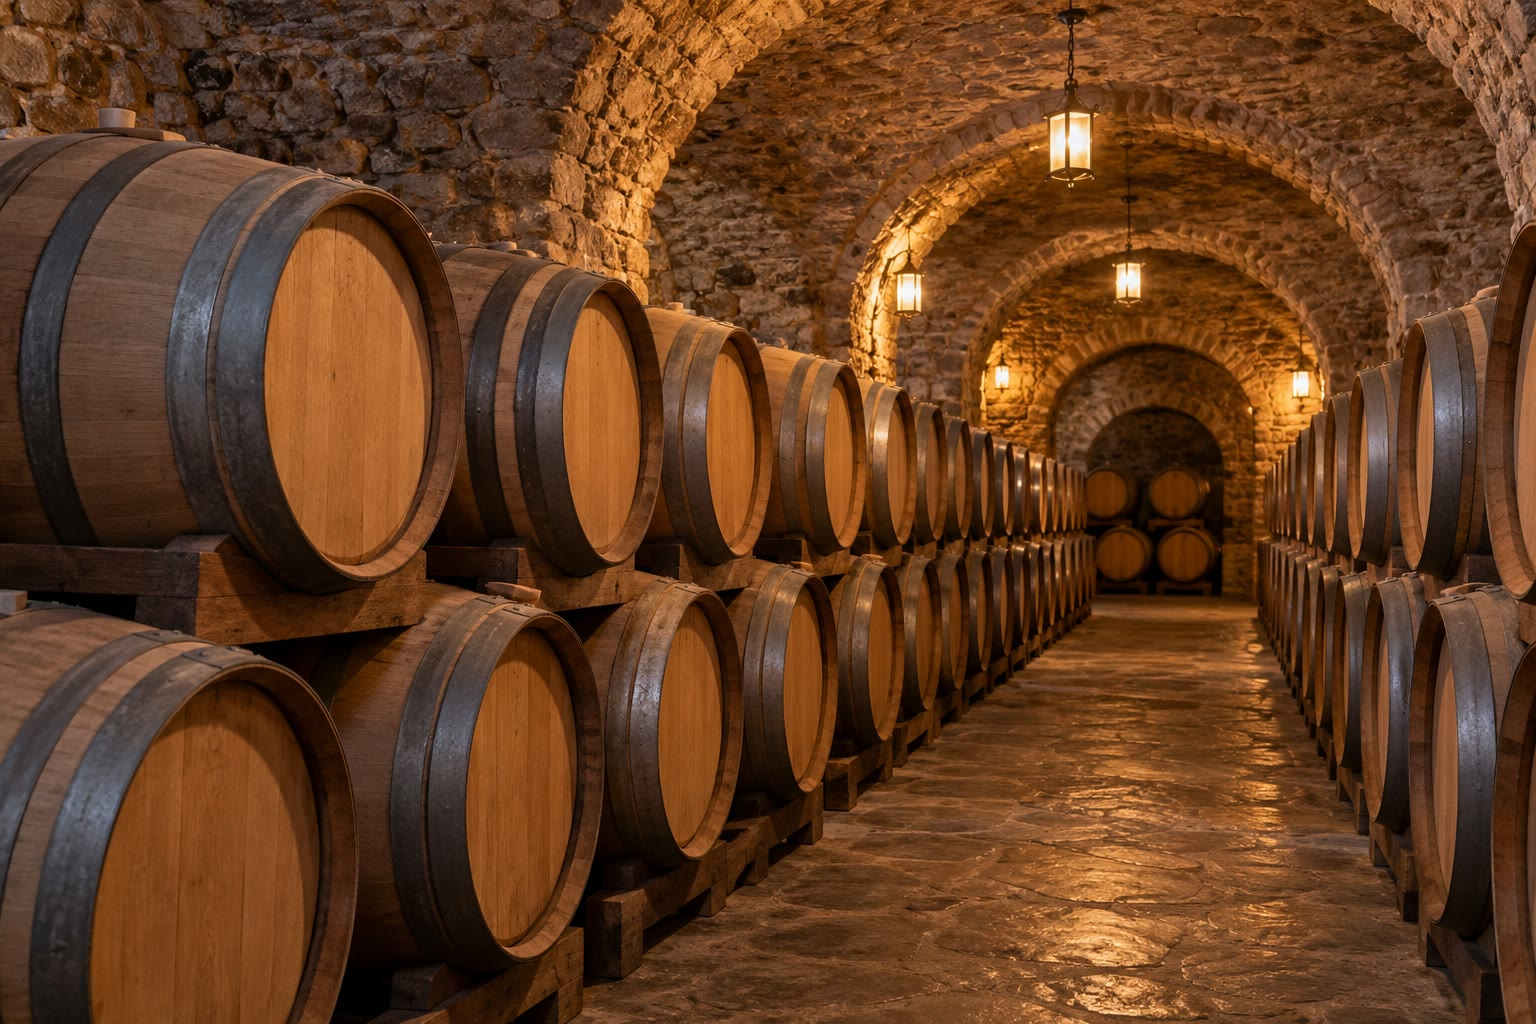
\includegraphics[width=0.58\linewidth]{images/book2/ai/b1-24-wine-cellar.jpg}

{\small Du vin qui vieillit en cave. À l'abri de l'air, le vin garde
son éthanol~; exposé à l'air, des bactéries acétiques l'oxydent en acide
éthanoïque.}
\end{omfigure}

\section{Les niveaux d'oxydation du carbone}

\begin{definition}[Niveau d'oxydation]\label{def:b1:organic-redox:oxidation-level}
Le \emph{niveau d'oxydation}\index{niveau d'oxydation} d'un atome de
carbone est son \omterm{def:b1:nernst:oxidation-number}{nombre d'oxydation}, obtenu par les règles de la
\cref{prop:b1:nernst:on-rules}~: chaque liaison à un atome plus
électronégatif (O, N, halogène) compte $+1$, chaque liaison à
l'hydrogène $-1$, chaque liaison à un autre carbone 0 (une double
liaison compte deux fois).
\end{definition}

\begin{proposition}[Nombres d'oxydation du carbone]\label{prop:b1:organic-redox:on-of-carbon}
Le \omterm{def:b1:nernst:oxidation-number}{nombre d'oxydation} d'un carbone est égal au nombre de liaisons à O, N
ou aux halogènes, diminué du nombre de liaisons à H. Au sein d'une même
famille de composés de même squelette carboné, la suite alcool $\to$
aldéhyde ou cétone $\to$ acide carboxylique $\to$ dioxyde de carbone est
une série d'oxydations à deux électrons chacune.
\end{proposition}

\begin{proof}
On rompt chaque liaison en donnant les deux électrons au partenaire le
plus électronégatif~: face à H (moins électronégatif que C), le carbone
gagne un électron, charge $-1$ par liaison C--H~; face à O, N ou un
halogène (plus électronégatifs), il en perd un, $+1$ par liaison~; les
liaisons C--C sont partagées également. En passant de \ce{-CH2OH}
($-1$ pour un carbone lié à un seul autre carbone) à \ce{-CHO} ($+1$),
puis à
\ce{-COOH} ($+3$), le nombre augmente de 2 à chaque étape~: deux
électrons.
\end{proof}

\begin{omfigure}
\begin{tikzpicture}[font=\small, >={Stealth}]
  \foreach \x/\f/\n in {0/\ce{CH4}/-4, 2.4/\ce{CH3OH}/-2, 4.8/\ce{HCHO}/0, 7.2/\ce{HCOOH}/+2, 9.6/\ce{CO2}/+4} {
    \node[draw, rounded corners, minimum width=1.5cm] at (\x,0) {\f};
    \node[below] at (\x,-0.5) {$\n$};
  }
  \foreach \x in {0.8,3.2,5.6,8.0} \draw[->, thick, omThm] (\x,0) -- ++(0.8,0);
  \node[omThm, above] at (4.8,0.5) {oxydation~: $-2\,\mathrm{e^-}$ (et $-2\,\ce{H+}$) à chaque étape};
  \node[left] at (-0.9,-0.75) {n.o. de C~:};
\end{tikzpicture}

{\small Les \omterm{def:b1:organic-redox:oxidation-level}{niveaux d'oxydation} de la famille à un carbone~: méthane,
méthanol, méthanal, acide méthanoïque, dioxyde de carbone. Chaque flèche
est une oxydation à deux électrons~; lue à rebours, une réduction.}
\end{omfigure}

\begin{method}[Équilibrer une demi-équation organique]\label{met:b1:organic-redox:balance-organic-redox}
\begin{enumerate}
  \item Écrire l'\omterm{def:b1:nernst:couple}{oxydant} et le \omterm{def:b1:nernst:couple}{réducteur} organiques avec le même
        squelette.
  \item Compter les électrons d'après la variation des \omterm{def:b1:nernst:oxidation-number}{nombres
        d'oxydation} des carbones qui changent (ou plus simplement~: deux
        par paire de H perdue, ou par O gagné).
  \item Équilibrer l'oxygène avec l'eau, l'hydrogène avec \ce{H+}, la
        charge avec les électrons.
\end{enumerate}
De l'éthanol à l'acide éthanoïque~: \ce{CH3CH2OH + H2O -> CH3COOH + 4H+ + 4e-}.
Avec le dichromate acidifié (\ce{Cr2O7^2- + 14H+ + 6e- -> 2Cr^3+ + 7H2O}),
trois molécules d'éthanol pour deux ions dichromate~:
\ce{3CH3CH2OH + 2Cr2O7^2- + 16H+ -> 3CH3COOH + 4Cr^3+ + 11H2O}.
\end{method}

\section{L'oxydation des alcools}

\begin{proposition}[Ce que donnent les alcools par oxydation]\label{prop:b1:organic-redox:alcohol-oxidation}
Un alcool primaire \ce{RCH2OH} est oxydé en aldéhyde \ce{RCHO}, puis
(dans l'eau, avec un \omterm{def:b1:nernst:couple}{oxydant} fort) en acide carboxylique \ce{RCOOH}~; un
alcool secondaire \ce{R2CHOH} en cétone \ce{R2CO}, qui résiste à une
oxydation ultérieure~; un alcool tertiaire \ce{R3COH} n'est pas oxydé
sans rupture d'une liaison C--C.
\end{proposition}

\begin{proof}
L'oxydation de l'alcool enlève l'hydrogène du OH et un hydrogène du
carbone fonctionnel, en formant C=O. Le carbone fonctionnel d'un alcool
tertiaire ne porte pas un tel hydrogène. L'aldéhyde porte encore un H
sur le carbone du carbonyle~; dans l'eau, il est en partie hydraté,
\ce{RCH(OH)2}, et cet hydrate est oxydé à son tour de la même façon en
\ce{RCOOH}. Une cétone n'a pas de H sur ce carbone et s'arrête là.
\end{proof}

Les \omterm{def:b1:nernst:couple}{oxydants} forts en solution aqueuse --- dichromate de potassium
acidifié ou permanganate --- oxydent les alcools primaires en acides.
Pour s'arrêter à l'aldéhyde, on le distille au fur et à mesure de sa
formation (les aldéhydes, dépourvus de \omterm{def:b1:intermolecular-forces-solvents:hbond}{liaisons hydrogène} O--H, bouillent à
plus basse température que les alcools dont ils proviennent), ou l'on
emploie des réactifs anhydres plus doux, décrits dans le volume de
deuxième année.

\begin{safety}{\ghs[5mm]{GHS03}\,\ghs[5mm]{GHS05}\,\ghs[5mm]{GHS06}\,\ghs[5mm]{GHS07}\,\ghs[5mm]{GHS08}\,\ghs[5mm]{GHS09}}
Le dichromate de potassium, l'\omterm{def:b1:nernst:couple}{oxydant} orange classique des alcools, est
classé parmi les substances susceptibles de provoquer le cancer~: on ne
le manipule qu'en petites quantités, avec gants et lunettes, et ses
déchets chromés sont collectés à part~; on lui préfère, quand c'est
possible, un \omterm{def:b1:nernst:couple}{oxydant} moins dangereux.
% ledger: ghs:K2Cr2O7
\end{safety}

\section{La réduction des composés carbonylés par les hydrures}

\begin{definition}[Donneur d'hydrure]\label{def:b1:organic-redox:hydride-donor}
Un \emph{donneur d'hydrure}\index{donneur d'hydrure} transfère un atome
d'hydrogène avec son \omterm{def:b1:lewis-resonance-vsepr:lewis}{doublet liant}, \ce{H-}, à un carbone \omterm{def:b1:electronic-effects:nucleophile}{électrophile}.
Le borohydrure de sodium \ce{NaBH4} et l'aluminohydrure de lithium
\ce{LiAlH4} sont des \emph{hydrures métalliques
complexes}\index{hydrure metallique complexe@hydrure métallique complexe}~: l'hydrure est
transféré depuis l'ion \ce{BH4-} ou \ce{AlH4-}, et non sous forme d'ion
libre.
\end{definition}

\begin{omfigure}
\setchemfig{atom sep=2.1em}
\schemestart
\chemfig{H_3B^{-}-[@{bh}]@{h}H}
\+
\chemfig{@{c}C(-[:150]R)(-[:210]R')=[@{co}]@{o}O}
\arrow{->}
\chemfig{C(-[:150]R)(-[:210]R')(-[2]H)-O^{-}}
\arrow{->[\ce{H2O}]}
\chemfig{C(-[:150]R)(-[:210]R')(-[2]H)-OH}
\schemestop
\chemmove{\draw[->, thick, shorten <=2pt, shorten >=3pt](bh) .. controls +(80:9mm) and +(180:7mm) .. (c);
          \draw[->, thick, shorten <=2pt, shorten >=2pt](co) .. controls +(90:6mm) and +(90:6mm) .. (o);}
\par\vspace{6pt}

{\small Réduction d'une cétone par le borohydrure~: un doublet B--H
forme la nouvelle liaison C--H tandis que le doublet $\pi$ de C=O passe
sur l'oxygène~; l'\omterm{def:b1:alcohol-activation:alkoxide}{alcoolate} est protoné par le solvant (eau ou alcool)
ou lors de l'hydrolyse. Chaque ion \ce{BH4-} peut céder successivement
ses quatre hydrogènes.}
\end{omfigure}

\begin{proposition}[Domaine d'action des deux hydrures]\label{prop:b1:organic-redox:hydride-scope}
Le borohydrure de sodium, employé dans l'eau ou dans les alcools, réduit
les aldéhydes en alcools primaires et les cétones en alcools
secondaires, et laisse intacts les esters, les acides carboxyliques, les
amides et les doubles liaisons C=C. L'aluminohydrure de lithium,
employé dans l'éther anhydre, réduit en outre les esters et les acides
carboxyliques en alcools primaires, et réagit violemment avec l'eau.
\end{proposition}

\begin{proof}
La liaison Al--H est plus polarisée que la liaison B--H (l'aluminium est
moins électronégatif que le bore)~; \ce{AlH4-} est donc un \omterm{def:b1:organic-redox:hydride-donor}{donneur
d'hydrure} bien plus fort, capable d'attaquer le carbonyle moins
\omterm{def:b1:electronic-effects:nucleophile}{électrophile} des esters et des carboxylates~; la même réactivité le fait
réagir avec tout hydrogène acide, y compris celui de l'eau. \ce{BH4-} ne
réagit que lentement avec l'eau et les alcools, et n'attaque que les
carbonyles les plus \omterm{def:b1:electronic-effects:nucleophile}{électrophiles}. Une liaison C=C isolée n'est pas
\omterm{def:b1:electronic-effects:nucleophile}{électrophile} et n'est réduite par aucun des deux.
\end{proof}

\section{La sélectivité}

\begin{definition}[Réaction chimiosélective]\label{def:b1:organic-redox:chemoselective}
Une \emph{réaction chimiosélective}\index{reaction chimioselective@réaction chimiosélective}
agit sur un groupe fonctionnel d'une molécule en présence d'autres
groupes qui pourraient, avec un autre réactif, réagir eux aussi.
\end{definition}

\begin{omfigure}
\begin{tabular}{lcc}
\hline
groupe & \ce{NaBH4} (solvant alcool) & \ce{LiAlH4} (éther anhydre) \\
\hline
aldéhyde \ce{RCHO} & alcool primaire & alcool primaire \\
cétone \ce{R2CO} & alcool secondaire & alcool secondaire \\
ester \ce{RCOOR} & pas de réaction & deux alcools \\
acide carboxylique \ce{RCOOH} & pas de réaction (sel) & alcool primaire \\
alcène \ce{C=C} & pas de réaction & pas de réaction \\
\omterm{def:b1:acetals-protection:hemiacetal}{acétal} & pas de réaction & pas de réaction \\
\hline
\end{tabular}

\smallskip
{\small Ce que réduisent les deux hydrures. Le borohydrure de sodium est
le réactif chimiosélectif~; l'aluminohydrure de lithium, le réactif
puissant.}
\end{omfigure}

\begin{example}[Un céto-ester]\label{ex:b1:organic-redox:ketoester}
Le 4-oxopentanoate d'éthyle, \ce{CH3CO(CH2)2COOEt}, donne avec le
borohydrure de sodium le 4-hydroxypentanoate d'éthyle~: seule la cétone
est réduite. Avec l'aluminohydrure de lithium, les deux groupes sont
réduits~: pentane-1,4-diol (et éthanol). Pour ne réduire que l'ester,
il faut d'abord protéger la cétone sous forme d'\omterm{def:b1:acetals-protection:hemiacetal}{acétal}
(\cref{ch:b1:acetals-protection}).
\end{example}

\begin{inthelab}[Réduire une cétone]
On ajoute le borohydrure de sodium par petites portions à une solution
froide de la cétone dans l'éthanol~: la réaction est exothermique, et du
dihydrogène se dégage de la lente réaction du réactif avec le solvant.
Après agitation, un acide dilué détruit l'excès de réactif (encore du
dihydrogène~: pas de flamme à proximité) et l'on extrait l'alcool.
L'aluminohydrure de lithium, au contraire, ne s'emploie que dans l'éther
anhydre sous gaz inerte, et son excès est détruit avec beaucoup de
précautions.
\end{inthelab}

\section{Exercices}

\begin{exercise}[$\star$]\label{exo:b1:organic-redox:1}
Donner le \omterm{def:b1:nernst:oxidation-number}{nombre d'oxydation} de chaque carbone dans l'éthanol,
l'éthanal, l'acide éthanoïque, la propanone et l'acide méthanoïque.
\end{exercise}

\begin{exercise}[$\star$]\label{exo:b1:organic-redox:2}
Que donne le dichromate acidifié avec le propan-1-ol, le propan-2-ol et
le 2-méthylpropan-2-ol~?
\end{exercise}

\begin{exercise}[$\star$]\label{exo:b1:organic-redox:3}
Écrire les \omterm{def:b1:nernst:couple}{demi-équations} des couples propanone/propan-2-ol et
éthanal/éthanol en milieu acide.
\end{exercise}

\begin{exercise}[$\star$]\label{exo:b1:organic-redox:4}
Que donnent le borohydrure de sodium et l'aluminohydrure de lithium avec
le butanal, la butanone, le butanoate d'éthyle et l'acide butanoïque~?
\end{exercise}

\begin{exercise}[$\star\star$]\label{exo:b1:organic-redox:5}
Équilibrer l'oxydation du propan-2-ol par le permanganate en milieu
acide (\ce{MnO4-}/\ce{Mn^2+}) et calculer le volume de permanganate à
\qty{0.020}{mol/L} nécessaire pour \qty{1.20}{g} d'alcool ($M = \qty{60.0}{g/mol}$).
\end{exercise}

\begin{exercise}[$\star\star$]\label{exo:b1:organic-redox:6}
Comment obtenir le propanal à partir du propan-1-ol sans qu'il soit
oxydé davantage~? Utiliser les températures d'ébullition~: propan-1-ol
\qty{97}{\celsius}, propanal
\qty{48}{\celsius}.
% ledger: bp:propanal, bp:propan-1-ol
\end{exercise}

\begin{exercise}[$\star\star$]\label{exo:b1:organic-redox:7}
Écrire le mécanisme de la réduction de l'éthanal par \ce{BH4-} dans
l'éthanol. Quel atome du produit provient du réactif~?
\end{exercise}

\begin{exercise}[$\star\star$]\label{exo:b1:organic-redox:8}
La réduction de la butanone par \ce{NaBH4} donne un alcool \omterm{def:b1:stereochemistry-in-depth:stereocentre}{chiral}.
Est-il optiquement actif~? Pourquoi~?
\end{exercise}

\begin{exercise}[$\star\star$]\label{exo:b1:organic-redox:9}
Dans l'éthylotest autrefois utilisé par la police, le dichromate orange
virait au vert. Écrire la réaction avec l'éthanol et expliquer le
changement de couleur.
\end{exercise}

\begin{exercise}[$\star\star\star$]\label{exo:b1:organic-redox:10}
Proposer des synthèses~: du 2-méthylbutan-2-ol à partir de l'éthanal et
d'un \omterm{def:b1:organomagnesium:organometallic}{organomagnésien}, suivis d'une oxydation et d'une seconde étape de
Grignard~; du pentan-3-ol à partir du propanal. Compter les oxydations
et les réductions.
\end{exercise}

\begin{exercise}[$\star\star\star$]\label{exo:b1:organic-redox:11}
Réduire seulement le groupe ester du 4-oxopentanoate de méthyle,
\ce{CH3CO(CH2)2COOCH3}. Planifier les trois étapes avec une \omterm{def:b1:acetals-protection:protecting-group}{protection} et
donner le produit.
\end{exercise}

\begin{exercise}[$\star\star\star$]\label{exo:b1:organic-redox:12}
Montrer, par les \omterm{def:b1:nernst:oxidation-number}{nombres d'oxydation} et par la \omterm{def:b1:nernst:couple}{demi-équation}, que
l'oxydation d'un alcool primaire en acide échange quatre électrons.
Généraliser à l'oxydation du méthane en dioxyde de carbone.
\end{exercise}

\section{Problème~: du cyclohexanol à l'acide adipique}

\begin{problem}[{Problème du week-end --- niveaux d'oxydation dans le
cyclohexanol, la cyclohexanone et l'acide adipique, l'oxydation par
l'acide nitrique et ses électrons, une voie au peroxyde d'hydrogène, et
la masse de protoxyde d'azote libérée par tonne d'acide adipique}]
\label{pb:b1:organic-redox:1}
L'acide adipique, ou acide hexanedioïque \ce{HOOC(CH2)4COOH}, est
fabriqué à grande échelle pour les nylons, surtout par oxydation du
cyclohexanol (mêlé de cyclohexanone) par l'acide nitrique, qui libère du
protoxyde d'azote \ce{N2O}, un puissant gaz à effet de serre. Masses
molaires (\unit{g/mol})~: \ce{C6H12O} 100.0,
\ce{C6H10O} 98.0, \ce{C6H10O4} 146.0, \ce{N2O} 44.0, \ce{HNO3} 63.0,
\ce{H2O2} 34.0.

\medskip
\noindent\textbf{Partie I --- Les \omterm{def:b1:organic-redox:oxidation-level}{niveaux d'oxydation}.}
\begin{enumerate}
  \item Donner le \omterm{def:b1:nernst:oxidation-number}{nombre d'oxydation} de chaque carbone du cyclohexanol.
  \item Même question pour la cyclohexanone.
  \item Même question pour l'acide adipique.
  \item Quels carbones sont oxydés lors du passage du cyclohexanol à
        l'acide adipique, et quelle liaison est rompue~?
  \item Combien d'électrons une molécule de cyclohexanol perd-elle~?
  \item Pourquoi la cyclohexanone, une cétone, est-elle néanmoins oxydée
        davantage ici~?
\end{enumerate}

\medskip
\noindent\textbf{Partie II --- La voie nitrique.}
\begin{enumerate}[resume]
  \item Écrire la \omterm{def:b1:nernst:couple}{demi-équation} du cyclohexanol en acide adipique en
        milieu acide.
  \item Donner le \omterm{def:b1:nernst:oxidation-number}{nombre d'oxydation} de N dans \ce{HNO3} et dans
        \ce{N2O}.
  \item Écrire la \omterm{def:b1:nernst:couple}{demi-équation} du couple \ce{HNO3}/\ce{N2O}.
  \item Les combiner~; vérifier que l'on obtient
        \ce{C6H12O + 2HNO3 -> C6H10O4 + N2O + 2H2O}.
  \item Combien de moles d'électrons sont échangées par mole d'acide
        adipique~?
  \item Calculer la masse d'acide nitrique consommée par tonne d'acide
        adipique.
\end{enumerate}

\medskip
\noindent\textbf{Partie III --- Une voie au peroxyde d'hydrogène.}
\begin{enumerate}[resume]
  \item Écrire la \omterm{def:b1:nernst:couple}{demi-équation} du couple \ce{H2O2}/\ce{H2O}.
  \item Écrire et équilibrer l'oxydation du cyclohexanol en acide
        adipique par le peroxyde d'hydrogène.
  \item Calculer la masse de \ce{H2O2} par tonne d'acide adipique.
  \item Quel est le seul sous-produit~? Pourquoi dit-on cette voie plus
        verte~?
  \item Le peroxyde d'hydrogène doit être activé par un \omterm{def:b1:elementary-steps:catalyst}{catalyseur}. À
        l'aide de l'\cref{exo:b1:nernst:12}, expliquer pourquoi une
        oxydation thermodynamiquement favorisée peut tout de même en
        exiger un.
  \item Que ferait le borohydrure de sodium à la cyclohexanone~? Écrire
        la réaction.
\end{enumerate}

\medskip
\noindent\textbf{Partie IV --- Les masses et le gaz à effet de serre.}
\begin{enumerate}[resume]
  \item Calculer la quantité de matière d'acide adipique dans une tonne.
  \item Calculer la quantité de \ce{N2O} formée en même temps par la voie
        nitrique.
  \item Calculer la masse de cyclohexanol nécessaire par tonne, pour un
        \omterm{def:b1:extent-q-and-k:fractional-extent}{rendement} de \qty{95}{\percent}.
  \item Donner la masse de \ce{N2O} libérée par tonne d'acide adipique
        par la voie nitrique, en tonnes.
\end{enumerate}
\end{problem}
